%!TEX root = ./main.tex
\section{Overview}
\label{sec2}

\subsection{Defination of resugaring}
This subsection is partially similiar to original defination in\cite{resugaring}.
\begin{Def}[Resugaring]
Given core language (named {\bfseries CoreLang}) and its evalation rules, together with surface language based on syntactic sugars of CoreLang (named {\bfseries Surflang}). For any expression of Surflang, getting the evaluation sequences of the expression in terms of SurfLang.\footnote{It's not strict, because we could allow some expressions in CoreLang shown.}
\end{Def}
For correctness of the resugaring, the evaluation sequences should maintain the following three properties:
\begin{enumerate}
\item {\bfseries Emulation} The evaluation sequences reflect the actual execution process.
\item {\bfseries Abstraction} The resugaring sequences should only contains terms in SurfLang, and each term of SurfLang should originate from initial expression.
\item {\bfseries Coverage} No sequence is skipped during the process.
\end{enumerate}

Given an example below.

For syntactic sugar {\bfseries and} and {\bfseries or}, the sugar rules are:
\begin{Codes}
(and e1 e2) \SurfStep{ (if e1 e2 \#f)}    \hfill (or e1 e2) \SurfStep{ (if e1 \#t e2)} 
\end{Codes}
% \begin{center}
% 	\parbox[t]{\textwidth}{%
% 		\begin{flushleft}  
% 			(and e1 e2) $\rightarrow$ (if e1 e2 \#f)\\
% 			(or e1 e2) $\rightarrow$ (if e1 \#t e2)
% 		\end{flushleft}  
% 	}%  
% \end{center}
which forms a simple SurfLang.

The evaluation rules of {\bfseries if} is:
\begin{Codes}
(if \#t e1 e2) \SurfStep{ e1} \\
(if \#f e1 e2) \SurfStep{ e2} 
\end{Codes}
% \begin{center}
% 	\parbox[t]{\textwidth}{%
% 		\begin{center}  
% 			if(\#t, e1, e2) → e1\\
% 			if(\#f, e1, e2) → e2
% 		\end{center}  
% 	}% 
% \end{center}

Then for SurfLang's expression $\mbox{and}(\mbox{or}(\#f, \#t), \mbox{and}(\#t, \#f))$ should get resugaring sequences as follow.

\begin{Codes}
    (and (or \#f \#t) (and \#t \#f))
\CoreStep (and \#t (and \#t \#f))
\CoreStep (and \#t \#f)
\CoreStep \#f
\end{Codes}
% \begin{figure}[ht]
% \parbox[t]{\textwidth}{
% 			\begin{center}  
% 				(and (or \#f \#t) (and \#t \#f))\\
% 				↓\\
% 				(and \#t (and \#t \#f))\\
% 				↓\\
% 				(and \#t \#f)\\
% 				↓\\
% 				\#f
% 			\end{center}  
% 		}
% \caption{resugaring example}
% \label{fig:example}
% \end{figure}

The reason we should get the sequences above is because $(\mbox{and}~(\mbox{or}~\#f~\#t)~(\mbox{and}~\#t~\#f))$ should desugar to $(\mbox{if}~(\mbox{if}~\#f~\#t~\#f)~(\mbox{if}~\#t~\#f~\#f)~\#f)$. Then in the CoreLang, the evaluation sequences will be as follow.
\begin{Codes}
    (if (if \#f \#t \#f) (if \#t \#f \#f) \#f)
\CoreStep (if \#t (if \#t \#f \#f) \#f)
\CoreStep (if \#t \#f \#f)
\CoreStep \#f
\end{Codes}
% \begin{figure}[ht]
% \parbox[t]{\textwidth}{
% 			\begin{center}  
% 				(if (if \#f \#t \#f) (if \#t \#f \#f) \#f)\\
% 				↓\\
% 				(if \#t (if \#t \#f \#f) \#f)\\
% 				↓\\
% 				(if \#t \#f \#f)\\
% 				↓\\
% 				\#f
% 			\end{center}  
% 		}
% \caption{evaluation sequences}
% \label{fig:coreseq}
% \end{figure}

The second item in the sequences can be desugared from $(\mbox{and}~\#t~(\mbox{and}~\#t~\#f))$, so resugars to it. So as the third item.

%Use a simple but sharp example to give an overview of your approach.
\subsection{Mixture Approach Framework}
We limit the language to s-expressions. Given an expression $\mbox{Exp} = (\mbox{Headid}~\mbox{Exp}*)$, the process of mixture approach will as Fig \ref{fig:mixture}.

\begin{figure}[t]
	\centering
	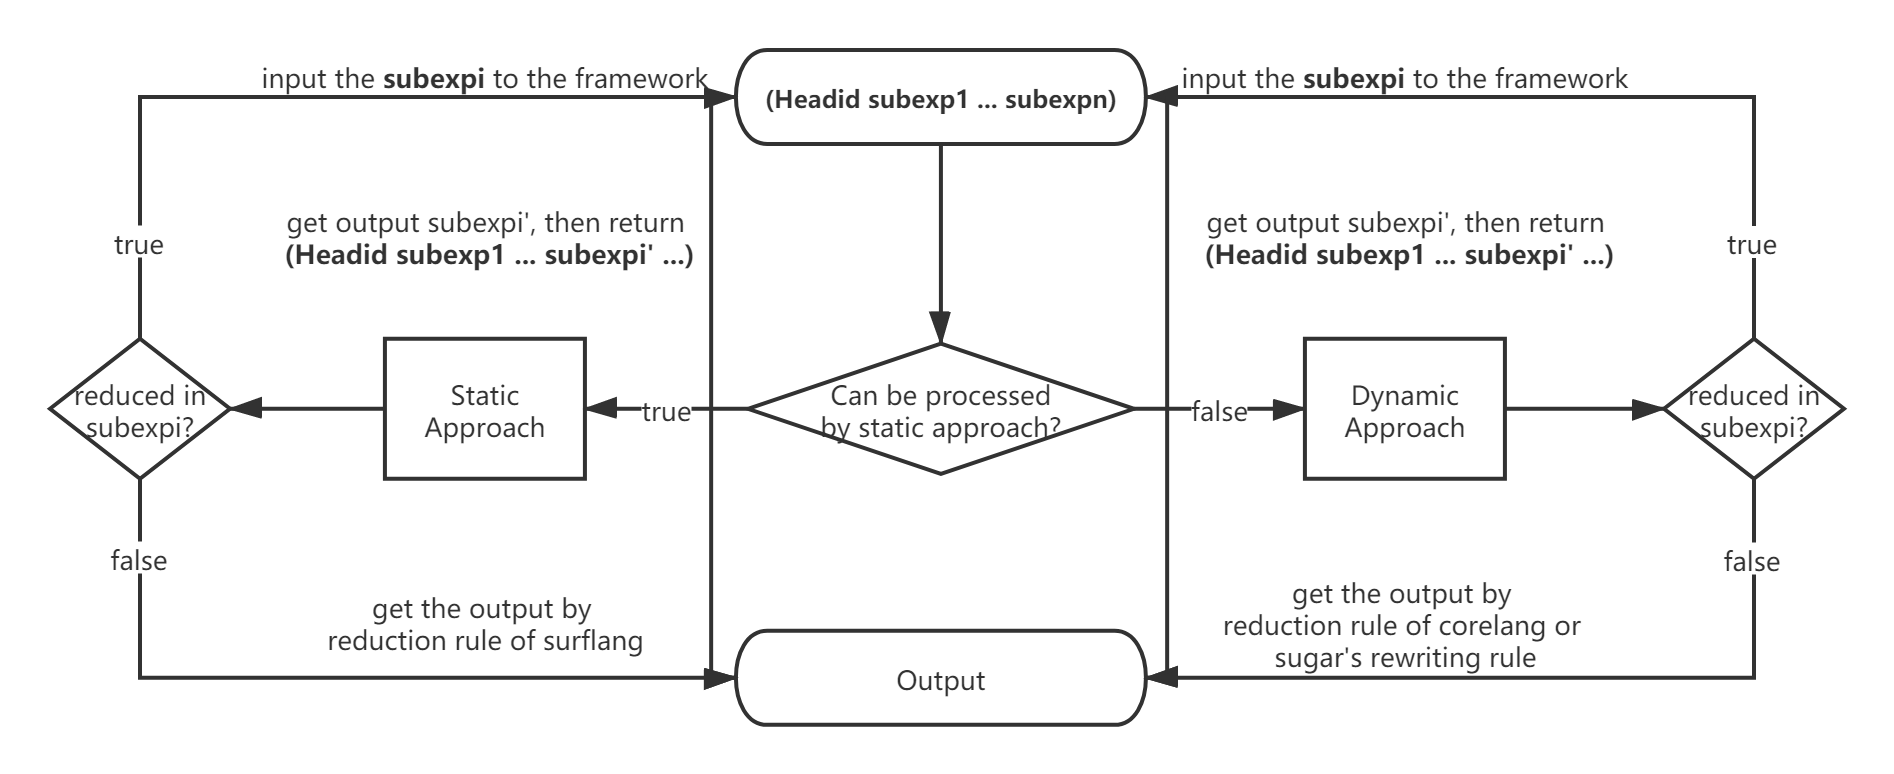
\includegraphics[width=12cm]{images/mixture.png}
	\caption{One step in framework of mixture approach}
	\label{fig:mixture}
\end{figure}

Given an example based on the former section. Besides sugar {\bfseries and}, {\bfseries or}, we add a recursive sugar {\bfseries mop} based on another new sugar {\bfseries op}. The recursive sugar can be handled by the dynamic approach, but not for the static one. (Reasons in later sections)
\begin{Codes}
\small{(op e1 e2)} \SurfStep{ (let x e1 (or x (and e2 x)))}
\small{(mop e lst)} \SurfStep{ (if (empty? lst) empty (cons (op e (first lst)) (mop e (rest lst))))} 
\end{Codes}

In the mop (map of op) sugar, we use both core language's term (such as {\bfseries if, empty?, cons, let, first, rest}) and existing syntactic sugar ({\bfseries and, or}). The semantics of core language is as common. But to show some exact step, we set the term {\bfseries cons} as a common expression (belonging to core language, but being displayed as surface language).


% For syntactic sugar {\bfseries and}, {\bfseries or} and {\bfseries map}, the sugar rules are:
% \begin{center}
% 	\parbox[t]{\textwidth}{%
% 		\begin{flushleft}  
% 			(and e1 e2) $\rightarrow$ (if e1 e2 \#f)\\
% 			(or e1 e2) $\rightarrow$ (if e1 \#t e2)\\
% 			(f e lst) $\rightarrow$ (if (empty? lst) empty (cons (let x e (or x (and (first lst) x))) (f e (rest lst))))
% 		\end{flushleft}  
% 	}%  
% \end{center}
% which forms a simple SurfLang.
If we execute 
\begin{Codes}
(mop \#t (list \#f \#t))
\end{Codes}
 the mixture approach will judge whether sugar mop can be handle by the static approach. No, then we use the dynamic approach in one step and get the intermidiate expression.
\begin{Codes}
(cons (op \#t (first (list \#f \#t))) (mop \#t (rest (list \#f \#t))))
\end{Codes}
Then according to semantics of {\bfseries cons}, the first subexpression should be reduced. The subexpression can be handled by the static approach, so getting a subsequence.
\begin{Codes}
	(cons (op \#t (first (list \#f \#t))) (mop \#t (rest (list \#f \#t))))
\CoreStep{(cons (op \#t \#f) (mop \#t (rest (list \#f \#t))))}
\CoreStep{(cons \#t (mop \#t (rest (list \#f \#t))))}
\end{Codes}
Then the second subexpression should be reduced, which is a recursive process. Finally, the subexpression (mop \#t (list)) will be processed by dynamic approach.
\begin{Codes}
	(mop \#t (list))
\SurfStep{ (if (empty? (list)) empty ...)}
\CoreStep{ empty}
\end{Codes}
Note that there are some steps should not be displayed, we define the common expressions above in syntaxs to restrict which intermediate step should be displayed.
% As we will see in Sec\ref{sec3}, the dynamic approach could handle recursive syntactic sugar, and the static approach could not. If we execute (f \#t (list \#f \#t)), the expression will Since the dynamic approach is more powerful and the static approach is more efficent, we should judge whether the input expression can be processed by static approach. If so, then use the static approach; if not, then use the dynamic approach to get (cons (let x \#t (or x (and (first (list \#f \#t)) x))) (f \#t (rest (list \#f \#t)))). Then the expression with headid {\bfseries cons} can be handled by static approach, which let the first subexpression reduced, so we get subsequences like (cons ... (f \#t (rest (list \#f \#t)))), (cons \#f (f \#t (rest (list \#f \#t)))). At this time, the static approach will let the second subexpression reduced, so the expression with headid {\bfseries f} will be processed by dynamic approach. (A recursive process it is.) 

The key idea of our dynamic approach, is that, regarding surface language and core language as a whole under the strategy of lazy desugaring. We design a core algorithm to choose the right reduction rule for any expression during the execution. Take the example $\mbox{and}(\mbox{or}(\#f, \#t), \mbox{and}(\#t, \#f))$ again. We will get the sequence as ...

\begin{figure}[ht]
\parbox[t]{\textwidth}{
			\begin{center}  
				(and (or \#f \#t) (and \#t \#f))\\
				~~~~~↓step1\\
				(and (if \#f \#t \#t) (and \#t \#f))\\
				~~~~~↓step2\\
				(and \#t (and \#t \#f))\\
				~~~~~↓step3\\
				(if \#t (and \#t \#f) \#f)\\
				~~~~~↓step4\\
				(and \#t \#f)\\
				~~~~~↓step5\\
				(if \#t \#f \#f)\\
				~~~~~↓step6\\
				\#f
			\end{center}  
		}
\caption{core-algo example}
\label{fig:core-algo}
\end{figure}

At step 1, we found the outermost $and$ sugar don't have to expand, because its first sub-expression will reduce earlier. At step 2, the same as step 1. At step 3, the outermost $and$ sugar have to expand, because no sub-expression will reduce after the whole expression desugar. At step 4, the inner $and$ sugar don't have to expand either. At step 5, the sugar have to desugar to CoreLang. Finally at step 6, we get the final result.

The key idea of our dynamic approach, is that, converting reduction semantics of core language into automata (called {\bfseries IFA}), building IFA for syntactic sugar, converting the IFA of sugars into reduction semantics. It is an abstract of dynamic approach in a sence, we will discuss it in Sec\ref{sec6}. Take another {\bfseries or} sugar for example.
\begin{flushleft}
	(or e1 e2) $\rightarrow$ (let x e1 (if x x e2))\\
	$(Or~e_1~e_2)$ $\rightarrow$ $(let~x~e_1~(if~x~x~e_2))$
\end{flushleft}  
The {\bfseries let} and {\bfseries if} expressions' reduction semantics can be represented as  the following automata.

\begin{tikzpicture}[->,>=stealth',shorten >=1pt,auto,node distance=2.8cm,
semithick]
\tikzstyle{every state}=[circle,draw,minimum size=16pt,font=\large]
 
\node[initial,state] (A) {$e_{1}$};
\node[state,accepting] (B) [above right of=A] {$e_{2}$};
\node[state,accepting] (C) [below right of=A] {$e_{3}$};
 
\path (A) edge node {\#t} (B)
edge node {\#f} (C)
edge [loop above] node {} (A)
;

\end{tikzpicture}


\begin{tikzpicture}[->,>=stealth',shorten >=1pt,auto,node distance=2.8cm,
semithick]
\tikzstyle{every state}=[circle,draw,minimum size=16pt,font=\large]
\node[initial,state] (A) {$e_{1}$};
\node[state,accepting](B)[right of=A,align=center, font=\small ]{$e\_2_{v}^{x}$}[above];
%\node at (-0.5,1)[draw, align=center]{example \\ example example};

\path[]
(A) edge node {$v$} (B)
(A) edge [loop above] node {} (2);

\end{tikzpicture}

Then for {\bfseries Or} sugar, we merge the IFA of if expression into node {$e_2$} of let's IFA.

\begin{tikzpicture}[->,>=stealth',shorten >=1pt,auto,node distance=2.8cm,
semithick]
\tikzstyle{every state}=[circle,draw,minimum size=16pt,font=\large]

\node[initial,state] (A) {$e_{1}$};
\node[state] (D) [right of=A,font=\small] {$x_{v}^{x}$};
\node[state,accepting] (B) [above right of=D,font=\small] {$x_{\#t}^{x}$};
\node[state,accepting] (C) [below right of=D] {$e_2$};

\path[]
(A) edge node {$v$} (D)
(A) edge [loop above] node {} (A)
(D) edge node {$\#t$} (B)
(D) edge node {$\#f$} (C);

\end{tikzpicture}

From the IFA of or expression, we can get the following reduction semantics.

\begin{flushleft}
\[\infer {(\mbox{Or}~e_1~e_2) \rightarrow (\mbox{Or}~e_1'~e_2)} {e_1~ \rightarrow~e_1'}  \]
\[(\mbox{Or}~\#t~e2) \rightarrow \#t \]
\[(\mbox{Or}~\#f~e2) \rightarrow e_2 \]
\end{flushleft}

Then the resugaring sequences can be get by the reduction semantics.